\documentclass{standalone}
\usepackage{tikz}
\usepackage{xcolor}
\usetikzlibrary{patterns, positioning}
\usetikzlibrary{shapes.misc}
\usepackage[outline]{contour}
\contourlength{1.5pt} 


\begin{document}
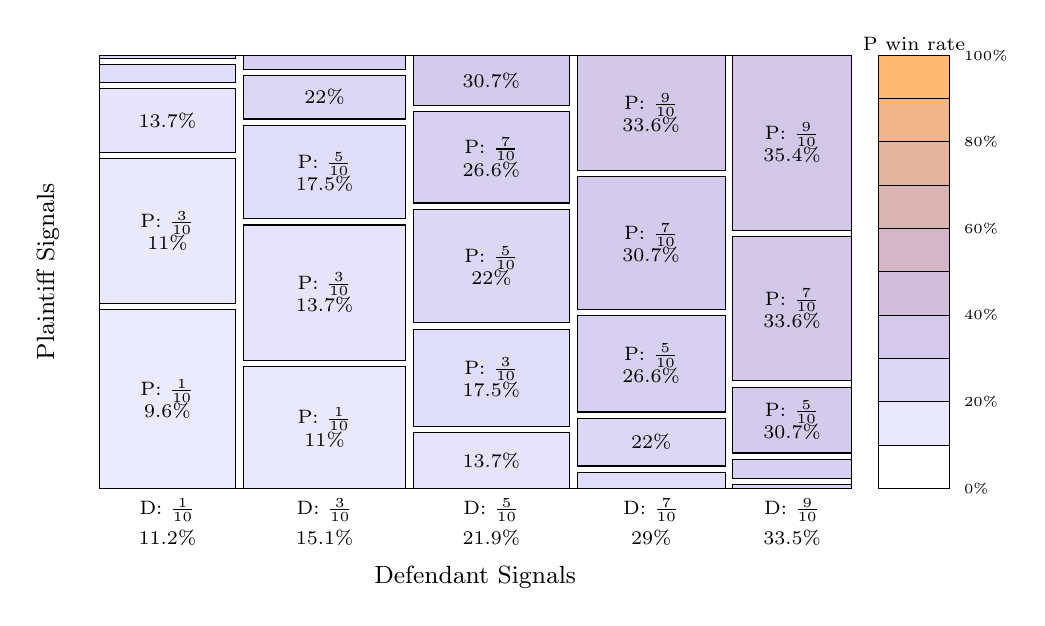
\begin{tikzpicture}
\newcommand{\DFractionOffset}{0.4}
\newcommand{\AxisLabelYAdjust}{-0.235}
\draw[draw=black] (0.6,2) rectangle (10.15,7.5);
\draw[fill=blue!90!orange!10!white!85!white, draw=black] (0.6,2) rectangle (2.3346,4.2713);
\draw (1.4672951280435742, 3.135640156361839) node[font=\scriptsize, text=black, align=center] {P: $\frac{1}{10}$\\ 9.6\%};
\draw[fill=blue!89!orange!11!white!84!white, draw=black] (0.6,4.3513) rectangle (2.3346,6.1875);
\draw (1.4672951280435742, 5.269410582941904) node[font=\scriptsize, text=black, align=center] {P: $\frac{3}{10}$\\ 11\%};
\draw[fill=blue!86!orange!14!white!83!white, draw=black] (0.6,6.2675) rectangle (2.3346,7.077);
\draw (1.4672951280435742, 6.672285598326043) node[font=\scriptsize, text=black, align=center] {13.7\%};
\draw[fill=blue!82!orange!18!white!82!white, draw=black] (0.6,7.157) rectangle (2.3346,7.3791);
\draw[fill=blue!78!orange!22!white!81!white, draw=black] (0.6,7.4591) rectangle (2.3346,7.5);
\draw (1.4672951280435742, 1.6) node[anchor=north, font=\scriptsize, text=black] {11.2\%};
\draw (1.4672951280435742, {1.6 + \DFractionOffset}) node[anchor=north, font=\scriptsize, text=black] {D: $\frac{1}{10}$};
\draw[fill=blue!89!orange!11!white!84!white, draw=black] (2.4346,2) rectangle (4.4914,3.5486);
\draw (3.462980059182164, 2.774307473560224) node[font=\scriptsize, text=black, align=center] {P: $\frac{1}{10}$\\ 11\%};
\draw[fill=blue!86!orange!14!white!83!white, draw=black] (2.4346,3.6286) rectangle (4.4914,5.3451);
\draw (3.462980059182164, 4.486850648890007) node[font=\scriptsize, text=black, align=center] {P: $\frac{3}{10}$\\ 13.7\%};
\draw[fill=blue!82!orange!18!white!82!white, draw=black] (2.4346,5.4251) rectangle (4.4914,6.6114);
\draw (3.462980059182164, 6.018247307480188) node[font=\scriptsize, text=black, align=center] {P: $\frac{5}{10}$\\ 17.5\%};
\draw[fill=blue!78!orange!22!white!81!white, draw=black] (2.4346,6.6914) rectangle (4.4914,7.2436);
\draw (3.462980059182164, 6.967515490646664) node[font=\scriptsize, text=black, align=center] {22\%};
\draw[fill=blue!73!orange!27!white!79!white, draw=black] (2.4346,7.3236) rectangle (4.4914,7.5);
\draw (3.462980059182164, 1.6) node[anchor=north, font=\scriptsize, text=black] {15.1\%};
\draw (3.462980059182164, {1.6 + \DFractionOffset}) node[anchor=north, font=\scriptsize, text=black] {D: $\frac{3}{10}$};
\draw[fill=blue!86!orange!14!white!83!white, draw=black] (4.5914,2) rectangle (6.5711,2.7093);
\draw (5.581220852400323, 2.3546323124250894) node[font=\scriptsize, text=black, align=center] {13.7\%};
\draw[fill=blue!82!orange!18!white!82!white, draw=black] (4.5914,2.7893) rectangle (6.5711,4.0218);
\draw (5.581220852400323, 3.4055196831115477) node[font=\scriptsize, text=black, align=center] {P: $\frac{3}{10}$\\ 17.5\%};
\draw[fill=blue!78!orange!22!white!81!white, draw=black] (4.5914,4.1018) rectangle (6.5711,5.5446);
\draw (5.581220852400323, 4.823195240473839) node[font=\scriptsize, text=black, align=center] {P: $\frac{5}{10}$\\ 22\%};
\draw[fill=blue!73!orange!27!white!79!white, draw=black] (4.5914,5.6246) rectangle (6.5711,6.7854);
\draw (5.581220852400323, 6.205011223678604) node[font=\scriptsize, text=black, align=center] {P: $\frac{7}{10}$\\ 26.6\%};
\draw[fill=blue!69!orange!31!white!78!white, draw=black] (4.5914,6.8654) rectangle (6.5711,7.5);
\draw (5.581220852400323, 7.182703353891223) node[font=\scriptsize, text=black, align=center] {30.7\%};
\draw (5.581220852400323, 1.6) node[anchor=north, font=\scriptsize, text=black] {21.9\%};
\draw (5.581220852400323, {1.6 + \DFractionOffset}) node[anchor=north, font=\scriptsize, text=black] {D: $\frac{5}{10}$};
\draw[fill=blue!82!orange!18!white!82!white, draw=black] (6.6711,2) rectangle (8.5491,2.2051);
\draw[fill=blue!78!orange!22!white!81!white, draw=black] (6.6711,2.2851) rectangle (8.5491,2.8899);
\draw (7.610092746396824, 2.5874810342265584) node[font=\scriptsize, text=black, align=center] {22\%};
\draw[fill=blue!73!orange!27!white!79!white, draw=black] (6.6711,2.9699) rectangle (8.5491,4.1935);
\draw (7.610092746396824, 3.5816788941433044) node[font=\scriptsize, text=black, align=center] {P: $\frac{5}{10}$\\ 26.6\%};
\draw[fill=blue!69!orange!31!white!78!white, draw=black] (6.6711,4.2735) rectangle (8.5491,5.9554);
\draw (7.610092746396824, 5.114468141950231) node[font=\scriptsize, text=black, align=center] {P: $\frac{7}{10}$\\ 30.7\%};
\draw[fill=blue!66!orange!34!white!77!white, draw=black] (6.6711,6.0354) rectangle (8.5491,7.5);
\draw (7.610092746396824, 6.767722275631989) node[font=\scriptsize, text=black, align=center] {P: $\frac{9}{10}$\\ 33.6\%};
\draw (7.610092746396824, 1.6) node[anchor=north, font=\scriptsize, text=black] {29\%};
\draw (7.610092746396824, {1.6 + \DFractionOffset}) node[anchor=north, font=\scriptsize, text=black] {D: $\frac{7}{10}$};
\draw[fill=blue!78!orange!22!white!81!white, draw=black] (8.6491,2) rectangle (10.15,2.0473);
\draw[fill=blue!73!orange!27!white!79!white, draw=black] (8.6491,2.1273) rectangle (10.15,2.369);
\draw[fill=blue!69!orange!31!white!78!white, draw=black] (8.6491,2.449) rectangle (10.15,3.286);
\draw (9.399556825135091, 2.867507077189732) node[font=\scriptsize, text=black, align=center] {P: $\frac{5}{10}$\\ 30.7\%};
\draw[fill=blue!66!orange!34!white!77!white, draw=black] (8.6491,3.366) rectangle (10.15,5.1986);
\draw (9.399556825135091, 4.2823189903185614) node[font=\scriptsize, text=black, align=center] {P: $\frac{7}{10}$\\ 33.6\%};
\draw[fill=blue!65!orange!35!white!76!white, draw=black] (8.6491,5.2786) rectangle (10.15,7.5);
\draw (9.399556825135091, 6.389304837573888) node[font=\scriptsize, text=black, align=center] {P: $\frac{9}{10}$\\ 35.4\%};
\draw (9.399556825135091, 1.6) node[anchor=north, font=\scriptsize, text=black] {33.5\%};
\draw (9.399556825135091, {1.6 + \DFractionOffset}) node[anchor=north, font=\scriptsize, text=black] {D: $\frac{9}{10}$};
\node[font=\small, text=black] at (5.375, {1.1 + \AxisLabelYAdjust}) {Defendant Signals};
\node[font=\small, text=black, rotate=90] at (-0.050000000000000044, 4.75) {Plaintiff Signals};
\draw[draw=black] (10.5,2) rectangle (11.4,7.5);
\draw (10.95, 7.65) node[font=\scriptsize, text=black] {P win rate};
\draw[fill=blue!100!orange!0!white!88!white, draw=black] (10.5,2) rectangle (11.4,2.55);
\draw[fill=blue!89!orange!11!white!84!white, draw=black] (10.5,2.55) rectangle (11.4,3.1);
\draw[fill=blue!78!orange!22!white!81!white, draw=black] (10.5,3.1) rectangle (11.4,3.65);
\draw[fill=blue!67!orange!33!white!77!white, draw=black] (10.5,3.65) rectangle (11.4,4.2);
\draw[fill=blue!56!orange!44!white!73!white, draw=black] (10.5,4.2) rectangle (11.4,4.75);
\draw[fill=blue!44!orange!56!white!70!white, draw=black] (10.5,4.75) rectangle (11.4,5.3);
\draw[fill=blue!33!orange!67!white!66!white, draw=black] (10.5,5.3) rectangle (11.4,5.85);
\draw[fill=blue!22!orange!78!white!62!white, draw=black] (10.5,5.85) rectangle (11.4,6.4);
\draw[fill=blue!11!orange!89!white!59!white, draw=black] (10.5,6.4) rectangle (11.4,6.95);
\draw[fill=blue!0!orange!100!white!55!white, draw=black] (10.5,6.95) rectangle (11.4,7.5);
\draw (11.46, 2) node[anchor=west, font=\tiny, text=black] {0\%};
\draw (11.46, 3.1) node[anchor=west, font=\tiny, text=black] {20\%};
\draw (11.46, 4.2) node[anchor=west, font=\tiny, text=black] {40\%};
\draw (11.46, 5.3) node[anchor=west, font=\tiny, text=black] {60\%};
\draw (11.46, 6.4) node[anchor=west, font=\tiny, text=black] {80\%};
\draw (11.46, 7.5) node[anchor=west, font=\tiny, text=black] {100\%};


\end{tikzpicture}
\end{document}